\documentclass[final]{beamer}

% ====================
% Packages
% ====================

\usepackage[T1]{fontenc}
\usepackage{lmodern}
\usepackage[size=custom,width=120,height=72,scale=1.0]{beamerposter}
\usetheme{gemini}
\usecolortheme{gemini}
\usepackage{graphicx}
\usepackage{booktabs}
\usepackage{tikz}
\usepackage{xcolor}
\usepackage{pgfplots}
\pgfplotsset{compat=1.7}

% ====================
% Lengths
% ====================

% If you have N columns, choose \sepwidth and \colwidth such that
% (N+1)*\sepwidth + N*\colwidth = \paperwidth
\newlength{\sepwidth}
\newlength{\colwidth}
\setlength{\sepwidth}{0.025\paperwidth}
\setlength{\colwidth}{0.3\paperwidth}

\newcommand{\separatorcolumn}{\begin{column}{\sepwidth}\end{column}}

% ====================
% Title
% ====================

\title{SINGLE-PARTICLE MOTION IN A WOBBLING NUCLEUS \\ A CASE-STUDY FOR ODD-MASS ISOTOPES}

\author{Robert Poenaru \inst{1,2} | \texttt{robert.poenaru@protonmail.ch}}

%\institute[shortinst]{\inst{1} Doctoral School of Physics, University of Bucharest, Bucharest, Romania \samelineand \inst{2} Department of Theoretical Physics, Horia-Hulubei National Institute of Nuclear Physics and Engineering, Bucharest-Magurele, Romania}

\institute[shortinst]{\inst{1} Doctoral School of Physics, University of Bucharest, Bucharest, Romania \\ \inst{2} Department of Theoretical Physics, Horia-Hulubei National Institute of Nuclear Physics and Engineering, Bucharest-Magurele, Romania}

% ====================
% Body
% ====================

\begin{document}

\addtobeamertemplate{headline}{} 
{\begin{tikzpicture}[remember picture, overlay]
     \node [anchor=north east, inner sep=0.9cm]  at (current page.north east)
     {
\includegraphics[height=11cm]{./images/logo.png}};
     \node [anchor=north west, inner sep=0.9cm]  at (current page.north west)
     {
\includegraphics[height=11cm]{./images/uniLogo.png}};
  \end{tikzpicture}}


\begin{frame}[t]
\begin{columns}[t]
\separatorcolumn

\begin{column}{\colwidth}

  \begin{block}{Introduction}

% Odd-mass triaxial nuclei are nuclear objects that lack spherical and axial symmetry, with some unique characteristics such as:
% \begin{itemize}
%     \item asymmetry between the moments of inertia associated with the principal axes of the ellipsoid
%     \item asymmetry in the mass and charge distributions
%     %\item rich energy spectra of collective character
%     %\item interactions between different states of predominately electric $E2$ type
%     \item unusually large deformations with respect to the $\beta_2$ shape parameter.
% \end{itemize}

In the present work, a description of the collective motion which occurs in odd-mass triaxial nuclei known as \textbf{Wobbling Motion} (WM) is done, using the \text{Particle Rotor Model} (PRM) \cite{bohr1998nuclear}. Within this framework, the total nuclear system consists of an even-even core and a \emph{valence} nucleon (also known as \emph{intruder}) which is moving in a quadrupole deformed mean-field, generated by the core. The strength of this deformed potential turns out to be a major player in driving the coupled system to different triaxial shapes.

\heading{Research goals}

\begin{enumerate}
    \item A quantitative analysis on the shapes of the deformation potential for several isotopes
    \item Comparison of the potential strength of nuclei at different quadrupole deformation and triaxiality parameters which dictate the nuclear shapes.
    %\item Determine now much does the \emph{odd-nucleon} contribute upon the excited spectra of the wobbling nuclei.
\end{enumerate}


  \end{block}

\begin{block}{Wobbling Motion}
  Wobbling motion in nuclei employs a \emph{precession} of the total angular momentum combined with an \emph{oscillation} of its projection onto the rotational axis. Different \emph{core-particle} couplings lead to different wobbling regimes (See Fig. \ref{wobbling-regimes}).
  \begin{figure}
      \centering
      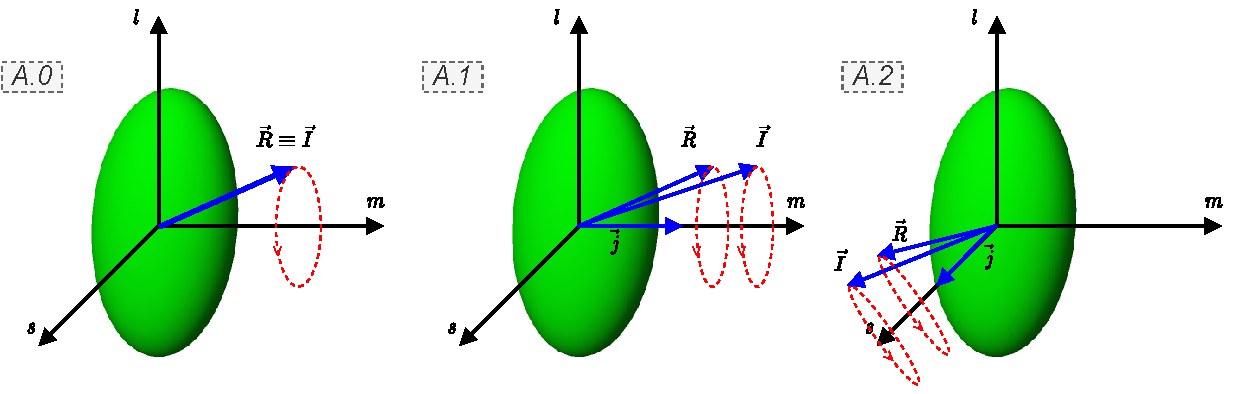
\includegraphics[scale=1.7]{images/wobbling_Regimes_COUPLING_SCHEME.pdf}
      \caption{An illustration with the wobbling regimes which can occur in a nucleus. From left to right: \emph{simple/ideal wobbler}, \emph{longitudinal wobbler}, \emph{transverse wobbler}.}
      \label{wobbling-regimes}
  \end{figure}
%   \begin{itemize}
%     \item a \emph{precession} of the total angular momentum combined with an \emph{oscillation} of its projection onto the rotational axis.
%     \item the precession + oscillation leads to \textbf{wobbling frequencies}: energy quanta of phononic type that will lead to collective excitations with harmonic-like structure in the nucleus  (See Fig. \ref{energy-function-min-point-evolution}-left).
%     \item different \emph{core-particle} couplings lead to different wobbling regimes (See Fig. \ref{wobbling-regimes}).
% \end{itemize}
 
 
\end{block}
\end{column}

\separatorcolumn

\begin{column}{\colwidth}

 \begin{figure}
\centering
\begin{minipage}{.5\textwidth}
  \centering
  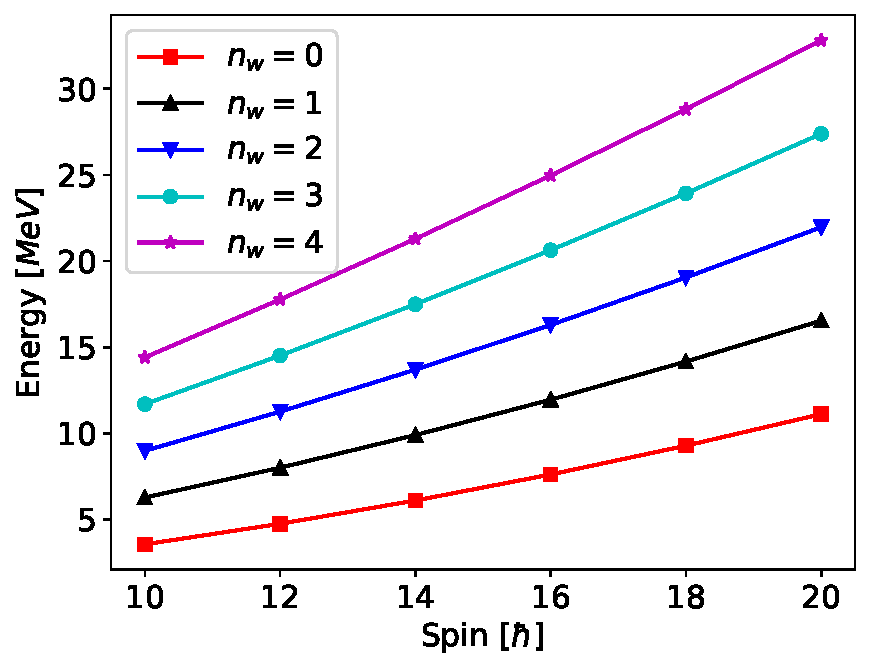
\includegraphics[scale=1]{images/simple_wobbling_spectrum.pdf}
\end{minipage}%
\begin{minipage}{.5\textwidth}
  \centering
 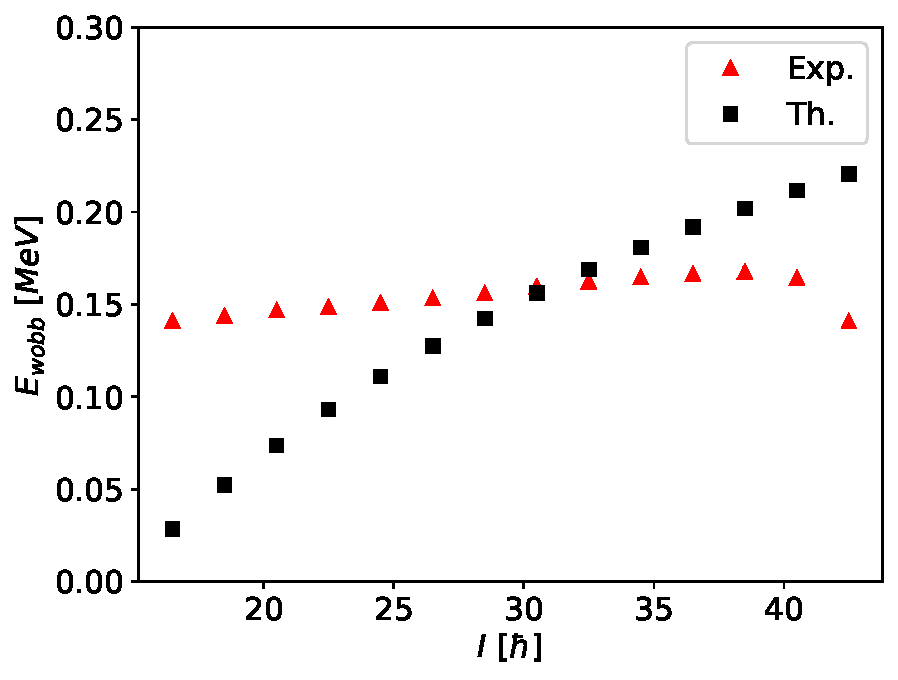
\includegraphics[scale=1]{images/wobbling_energy_ThExp.pdf}
\end{minipage}
\caption{\textbf{Left:} ideal wobbler (case $A.0$ depicted above). \textbf{Right:} real wobbling spectrum of $^{163}$Lu (case $A.2$ depicted above).}
    \label{energy-function-min-point-evolution}
\end{figure}
 
  \begin{block}{Single-Particle Deformed Potential}

The system is described by the total PRM Hamiltonian:
\begin{align}
    \hat{H}=\hat{H}_\text{core}+\hat{H}_\text{sp}\ ,
\end{align}
where $\hat{H}_\text{core}$ describes the dynamics of the triaxial core \cite{raduta2020new}, and $\hat{H}_\text{s.p.}$ is the single-particle potential that corresponds to the odd nucleon. Depending on the angular momentum $\vec{j}$ of the nucleon, and the strength parameter $V$, its expression corresponds to a Nilsson potential \cite{nilsson1955mat} as such:
\begin{align}
\hat{H}_\text{sp}&\equiv V_\text{sp}=\frac{\mathbf{V}}{j(j+1)}\left[\cos\gamma Y_{20}+\frac{\sin\gamma}{\sqrt{2}}\left(Y_{2-2}+Y_{22}\right)\right],\\
V&=\chi(A,\beta_2).
\end{align}


  \end{block}
  
    \begin{block}{Results}
  The deformed potential in which the valence nucleon is moving, with respect to different values of triaxial parameter $\gamma$ and quadrupole deformation can be seen in Fig. \ref{gamma-beta-dev-v}.
  \end{block}
  
\end{column}

\separatorcolumn

\begin{column}{\colwidth}
 \begin{figure}
     \centering
     \includegraphics[scale=1.05]{images/dp-Vsp-gammaDependece.pdf}
     
     \includegraphics[scale=1.06]{images/dp-Vsp-betaDependece.pdf}
     \caption{$V_\text{sp}$ for fixed $\beta_2$ (top) and fixed $\gamma$ (bottom). The odd nucleon's a.m. is $j=13/2\ \hbar$.}
     \label{gamma-beta-dev-v}
 \end{figure}
    % \begin{table}
    %   \centering
    %   \begin{tabular}{l c c c c}
    %     \toprule
    %     \textbf{Isotope} & \textbf{$\gamma$} & \textbf{$\beta_2$} & \textbf{$\mathbf{V}$} & $\vec{j}$\\
    %     \midrule
    %     Foo & 13.37 & 384,394 & \alpha &j \\
    %     Bar & 2.17 & 1,392 & \beta &j \\
    %     Baz & 3.14 & 83,742 & \delta &j \\
    %     Qux & 7.59 & 974 & \gamma &j \\
    %     \bottomrule
    %   \end{tabular}
    %   \caption{A table caption.}
    % \end{table}
  
    \begin{block}{Conclusions}
    \begin{itemize}
    \item The shape of the deformed potential is much more \emph{sensitive} with respect to  parameter $\gamma$.
    \item The strength parameter $V$ that characterizes the potential $V_\text{sp}$ has a specific shape.
    \end{itemize}
  \end{block}

  \begin{block}{References}

    \nocite{*}
    \tiny{\bibliographystyle{plain}\bibliography{poster}}

  \end{block}

\end{column}

\separatorcolumn

\end{columns}

\end{frame}

\end{document}